


\chapter{Экспериментальная часть}\label{exp}
%\addcontentsline{toc}{chapter}{4 Экспериментальная часть}

Оценка качества работы алгоритмов. Экспериментальное сравнение работы различных алгоритмов поиска расстояния Левейнштейна
(зависимость времени выполнения от длины слова).

\section{Примеры работы}\label{examples}

\begin{figure}[H]
    \center{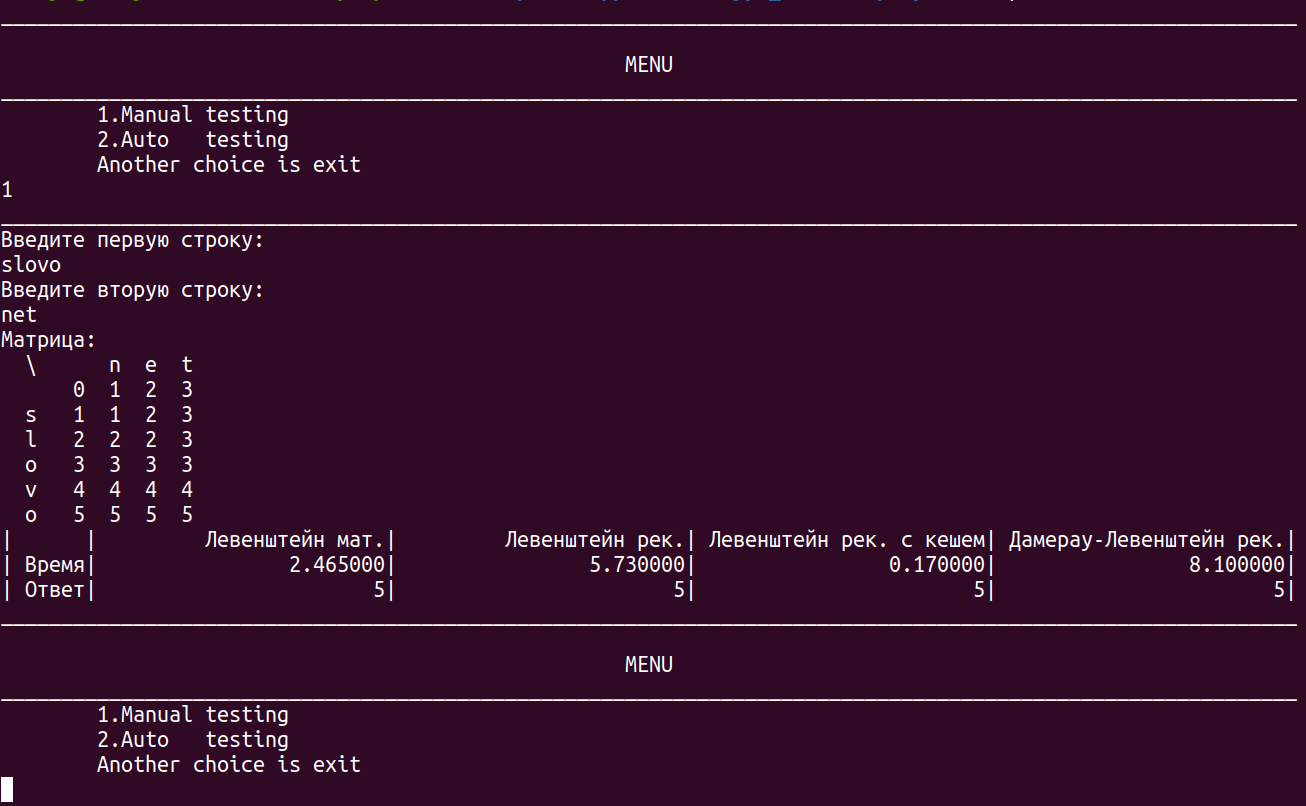
\includegraphics[scale=0.4]{workExample}}
    \caption{Ручное тестирование}
    \label{ris:work_example1}
  \end{figure}
  
\begin{figure}[H]
    \center{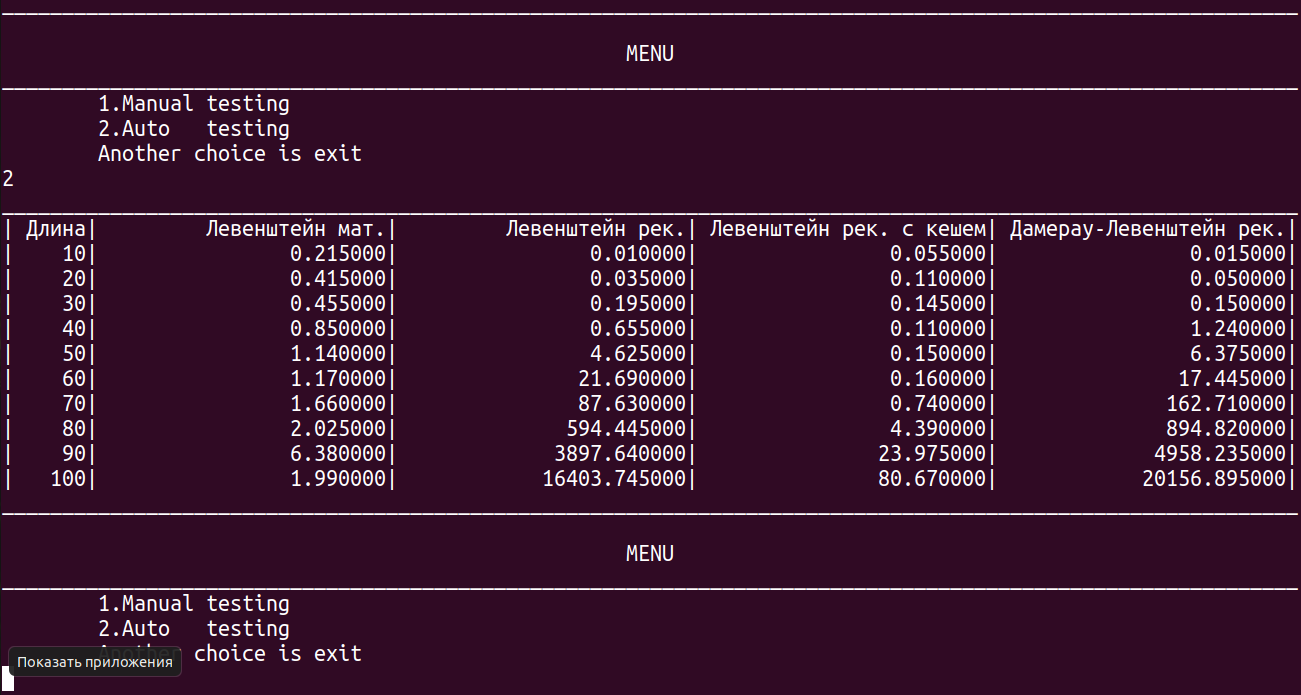
\includegraphics[scale=0.4]{workExample2}}
    \caption{Автоматическое тестирование}
    \label{ris:work_example2}
  \end{figure}

\section{Замеры времени}\label{experimentgraph}

На рисунках \ref{ris:graph1} и \ref{ris:graph2} показаны графические результаты сравнения исследуемых алгоритмов по времени. 

\begin{figure}[H]
    \center{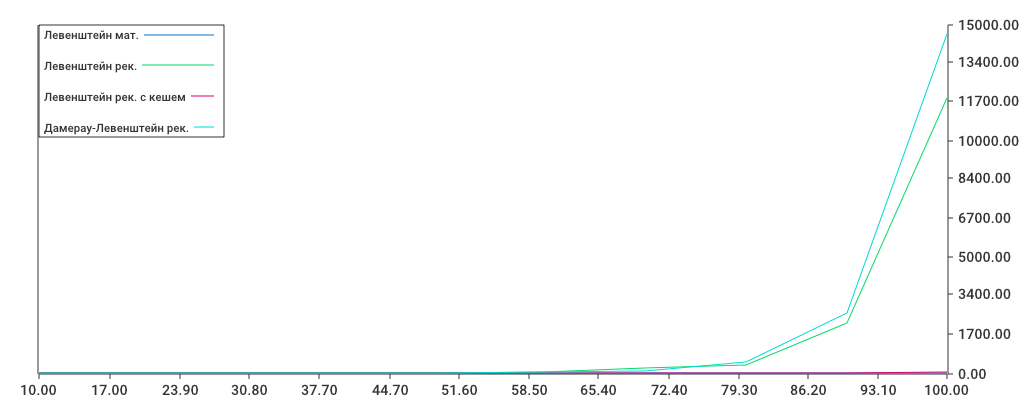
\includegraphics[scale=0.4]{../Lab1/output.png}}
    \caption{Сравнение всех 4 исследуемых алгоритмов по времени}
    \label{ris:graph1}
\end{figure}

\begin{figure}[H]
    \center{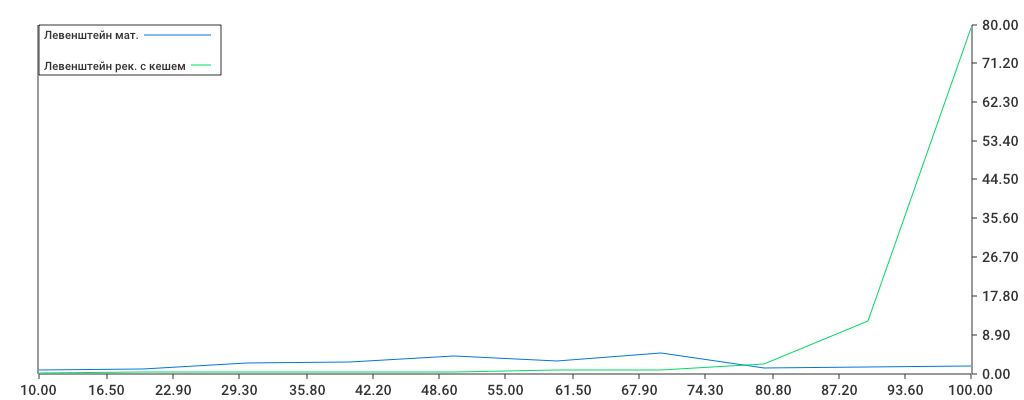
\includegraphics[scale=0.4]{../Lab1/output2.png}}
    \caption{Сравнение матричного и рекурсивного с кешем алгоритмов поиска расстояния Левенштейна}
    \label{ris:graph2}
\end{figure}


\section{Вывод экспериментальной части}\label{experimentresult}

Таким образом, по графикам подтвердилось предположение, что самый эффективный алгоритм поиска расстояния Левенштейна
из рассматриваемых в работе – рекурсивный метод с кешем. Рекурсивный алгоритм поиска расстояния Дамерау - Левенштейна дольше, чем 
рекурсивный алгоритм Левенштейна, что объясняется дополнительными операциями поиска перепутанных букв: (fd -> df).




\chapter{Заключение}\label{exit}

В данной работе был проведен обзор алгоритмов поиска расстояния Левенштейна и Дамерау-Левенштейна. 
Изучены алгоритмы поиска расстояния между строками: рекурсивные алгоритмы поиска расстояния Левенштейна 
и Дамерау-Левенштейна, рекурсивный алгоритм с кешем поиска расстояния Левенштейна, матричный алгоритм поиска Левенштейна. 
Получены практические навыки реализации исследуемых алгоритмов на языке программирования Go. 
Проведён сравнительный анализ алгоритмов по затрачиваемым ресурсам (зависимость времени от длины массива). 
Экспериментально подтверждены различия в эффективности алгоритмов с указанием лучших и худших случаев. 
При сравнении данных алгоритмов получены следующие результаты: самый эффективный алгоритм поиска расстояния Левенштейна 
из рассматриваемых в работе - рекурсивный алгоритм с кешем.


